\documentclass[final]{beamer}

\mode<presentation>
{
  %\definecolor{berkeleyblue}{HTML}{003A70}
  %\definecolor{berkeleygold}{HTML}{F2A900}
  \definecolor{berkeleyblue}{HTML}{003262}
  \definecolor{berkeleygold}{HTML}{FDB515}
%http://www.berkeley.edu/brand/img/downloads/UCB%20Brand%20Guidelines_FINAL_small.pdf
  \usetheme{I6dv}      % or try Darmstadt, Madrid, Warsaw, ...
  %\usecolortheme{dove} % or try albatross, beaver, crane, ...
  \setbeamercolor{structure}{fg=berkeleygold,bg=berkeleyblue}
  \setbeamercolor{palette primary}{fg=berkeleyblue,bg=berkeleygold} % changed this
  \setbeamercolor{palette secondary}{bg=berkeleyblue,fg=white} % changed this
  \setbeamercolor{palette tertiary}{bg=berkeleyblue,fg=white} % changed this
\setbeamercolor{bibliography item}{bg=white,fg=black}
\setbeamercolor{bibliography entry author}{bg=white,fg=black}
\setbeamercolor{bibliography entry journal}{bg=white,fg=black}
\setbeamercolor{bibliography entry note}{bg=white,fg=black}
  \usefonttheme{structurebold}  % or try serif, structurebold, ...
  \useinnertheme{circles}
  \setbeamertemplate{navigation symbols}{}
  \setbeamertemplate{footline}[title]{}
  \setbeamertemplate{footline}[author]{}
  \usebackgroundtemplate{
%  \tikz[overlay,remember picture] %Can insert a Berkeley watermark
%  \node[opacity=1, at=(current page.south west),anchor=south west, inner sep=2pt] {
%    \includegraphics[height=.5in,width=.5in]{img/ucseal_540_139.eps}};
}
}
%\renewcommand*{\bibfont}{\scriptsize}
\usepackage[sorting=none]{biblatex} 
  \usepackage{ragged2e}
  \usepackage{type1cm}
  \usepackage{calc} 
  \usepackage{times}
  \usepackage{amsmath,amsthm, amssymb, latexsym}
%  \boldmath
  \usepackage[english]{babel}
  \usepackage[latin1]{inputenc}
  \usepackage[orientation=landscape,size=a0,scale=1.4,debug]{beamerposter}
  \graphicspath{{img/}}
  %\title[Fancy Posters]{Making Really Fancy Posters with \LaTeX}
  %\author[Dreuw \& Deselaers]{Philippe Dreuw and Thomas Deselaers}
  %\institute[University of California, Berkeley]{Department of Nuclear Engineering}
  \newcommand{\footlinetext}{}
  \usepackage{biblatex}

% Transport equation stuff
\newcommand{\Sn}{\ensuremath{S_N}}
\newcommand{\Macro}{\ensuremath{\Sigma}}
\newcommand{\vOmega}{\ensuremath{\hat{\Omega}}}
\newcommand{\Ye}[2]{\ensuremath{Y^e_{#1}(\vOmega_#2)}}
\newcommand{\Yo}[2]{\ensuremath{Y^o_{#1}(\vOmega_#2)}}
\newcommand{\ve}[1]{\ensuremath{\mathbf{#1}}}

\setbeamertemplate{bibliography item}[text]
\addbibresource{2015-bascd.bib}
\renewcommand*{\bibfont}{\footnotesize}


\title[RQI with MGE]{RQI with a Multigrid in Energy Preconditioner for Massively Parallel Neutron Transport}
\author[R.N.\ Slaybaugh et al.]{R.N.\ Slaybaugh$^{1}$, T.M.\ Evans$^{2}$, G.G. Davidson$^{2}$, S.P.\ Hamilton$^{2}$}
  \institute[UC Berkeley]{$^{1}$Department of Nuclear Engineering, University of California, Berkeley\\
  $^{2}$Radiation Transport Group, Oak Ridge National Laboratory}
  \date{December 11, 2015}

\begin{document}
	\begin{frame}{}
%    \maketitle

%%%%%%%%%%%%%%
% FIRST COLUMN
%%%%%%%%%%%%%%

  		\begin{columns}[t]
    		\begin{column}{.3\linewidth}
    			\vfill
    			\begin{block}{\large Motivation}
      			\begin{itemize}
			\item{Nuclear reactor design, shielding, nuclear security}
			\item{3D deterministic calculations need fine resolution in space, 
			      energy, and angle}
			\item{Need to use supercomputing architectures effectively}
			\item{Three complimentary methods: multigroup (MG) block Krylov, 
			      Rayleigh quotient iteration (RQI), multigrid in energy (MGE)
			      preconditioner}
			\end{itemize}
    			\end{block}
    	\vfill
    			\begin{block}{\large Boltzmann Transport Equation}
			\begin{itemize}
	 		\item{Solve for $\psi$, the angular neutron flux (n/cm$^2$-s-steradian)}
	 		\begin{equation}
	 		  \ve{L}\psi = \ve{MS}\phi + \frac{1}{k}\ve{M}\chi \ve{f}^{T}\phi	                
	 		  \label{eq:eigenvalue}
	 		\end{equation}	 		
	 		\item{Collocation method in angle: $\phi = \mathbf{D} \psi$ (n/cm$^2$-s)}
	 		\item{$\ve{L}$ is the $\vOmega \cdot \nabla + \Macro_t$ operator; $\ve{M}$
	 		 projects $\phi$ onto discrete angles; $\ve{S}$
	 		 is the scattering matrix; $\ve{f}$ contains the fission source, 
	 		 $\nu \Macro_{f}$; and $k$ is the asymptotic ratio of the number of 
	 		 neutrons in one generation to the next}
	 		\item{Rearrange Eqn.~\eqref{eq:eigenvalue}; define $\ve{T} = \ve{DL}^{-1}$ 
	 		 and $\ve{F} = \chi \ve{f}^{T}$ \cite{denovo}}:
            \begin{equation}
              (\ve{I} - \ve{TMS})\phi = \frac{1}{k} \ve{TMF} \phi
              \label{eq:OperatorEvalForm}
            \end{equation}
            \item{Get series of ``within-group'' eqns., each only a function of space
             and angle}
            \item{Groups can be coupled by scattering from low to higher energy
             $\rightarrow$ iterative ``multigroup'' solves over the coupled portion needed}
			\end{itemize}
    			\end{block}
    	\vfill
        	\begin{block}{\large Multigroup Block Krylov \cite{Davidson2013}}		
		\begin{itemize}
		\item{Groups historically solved in series with Gauss Seidel} 
			\begin{figure}[h!]
			\centering
	      		\includegraphics{block-krylov.png}
			%\caption{MG Krylov group blocking}
			\end{figure}
		\item{In Denovo~\cite{denovo} solve downscatter groups individually}
		\item{Solve upscatter block together with multi-group-sized iteration vector 
		      in GMRES}
		\item{Enables parallelization in energy (``multisets")}
		\end{itemize}
        	\end{block}
    	\end{column}

%%%%%%%%%%%%%%%
% SECOND COLUMN
%%%%%%%%%%%%%%%

    \begin{column}{.3\linewidth}
    \begin{block}{Rayleigh Quotient Iteration \cite{Slaybaugh2012}}
	\begin{itemize}
	\item{Eigenvalues historically found with power iteration (PI)}
	\begin{equation}
	(\ve{I} - \ve{TMS})^{-1} \ve{TMF} \phi = k\phi
	\end{equation}
	\vspace*{-1em}
		\begin{itemize}
		\item{Error reduced as $\lambda_{2}/\lambda_{1}$; slow in many nuclear cases}
		\end{itemize}
		\vspace*{0.2 em}
	\item{Shifted inverse iteration (PI on $(\ve{P} - \mu \ve{I})^{-1}$) gives same eigenvectors; $\sigma([\ve{P} - \mu \ve{I}]^{-1}) = \{1/(\lambda - \mu):\lambda \in \sigma(\ve{P})\}$ }
		\vspace*{0.1 em}
		\begin{itemize}
		\item{Error now reduced as $(\lambda_{1}-\mu)/(\lambda_{2}-\mu)$}
		\end{itemize}		
		\vspace*{0.1 em}
	\item{RQI uses Rayleigh quotient as an \textit{optimal} shift}
		\begin{equation}
          \rho = \frac{(\ve{I} - \ve{TMS})\phi}{\ve{TMF} \phi} \approx \frac{1}{k}
		\end{equation}
		\item{RQI in Denovo: subtract $\rho \ve{TMF}$ from both sides of 
		 Eq.\ \eqref{eq:OperatorEvalForm}}
        \begin{equation}
          (\ve{I} - \ve{TM}\ve{\tilde{S}})\phi =( \gamma - \rho) \ve{TMF} \phi  \:, 
          \label{eq:OperatorShiftedEval} 
        \end{equation}
		\item{$\ve{\tilde{S}} \equiv \ve{S} + \rho\ve{F}$ is energy-block dense;
		 need MG Krylov}
		\item{The RQ shift can cause ill conditioning; difficult to converge
		 eigenvector iterations with Krylov}
	\end{itemize}
            \end{block}
		\vfill
        	\begin{block}{\large Multigrid in Energy \cite{Slaybaugh2013}}
        \begin{itemize}
			\item{Multigrid in Energy (MGE) as right preconditioner}
			\item{Relaxation method is weighted Richardson}
			\begin{equation}
              \phi^{m} = \bigr(\ve{I} + \omega(\ve{TMS} - \ve{I})\bigl)\phi^{m-1}
               + \omega b^{m-1}
            \label{eq:relax}
            \end{equation} 
			\item{Parallelization: each set restricts, prolongs, and relaxes only
			 its own groups; does not need to communicate with other energy sets
			 beyond for upscattering in the solver}
			\item{Can use reduced angular quadrature in the preconditioner}
			\end{itemize}
        	\end{block}
			\vfill
		\begin{block}{\large Results\textemdash Past Work 
		              \cite{Slaybaugh2012}, \cite{Slaybaugh2013}}
\begin{columns}
	\column{0.45\linewidth}
	\begin{figure}[h!]
	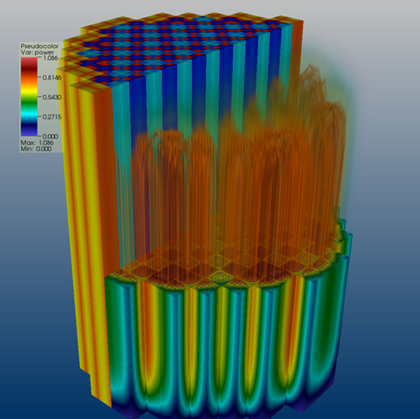
\includegraphics[width=5in]{../figs/denovo-pwr.png}
	\caption{\footnotesize Full PWR; $S_{12}$ (168 angle sets), 233,858,800 
	         cells, 44 groups: 1.73 trillion unknowns}
	\end{figure}
	\column{0.55\linewidth}
	\begin{itemize}
	\item{RQI could solve easy problems without preconditioning, but not hard ones}
	\item{Using a reduced quadrature set in MGE is highly valuable}
	\item{No need to have MGE restrict to 1 group, a few grids are sufficient}
	\item{MGE is not very helpful with PI}
	\item{MGE scales very well in energy}
	\end{itemize}
\end{columns}
\vspace*{0.5 em}
	\begin{itemize}
	\item{\textit{Will preconditioning with MGE facilitate the use of RQI?}}
	\item{\textit{Will the combination be better for some problems?}}
	\end{itemize}
		\end{block}
	\vfill
      \end{column}

%%%%%%%%%%%%%%
% THIRD COLUMN
%%%%%%%%%%%%%%

      \begin{column}{.3\linewidth}
		\begin{block}{Results - Jezebel with Artificial Boundary}
\begin{columns}
	\column{0.3\linewidth}
	\begin{figure}[h!]
	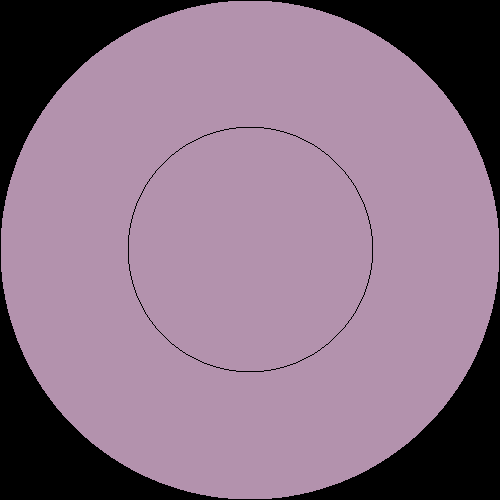
\includegraphics[width=4in]{img/jezebel-shells.png}
	\caption{Plot of ``jezebel" configuration with an inserted artificial boundary.}
	\end{figure}
	\column{0.7\linewidth}
	\begin{itemize}
	\item{Artificial boundary put in place to test different method speeds}
	\item{Verify that delta-tracking performs correctly with boundary}
	\end{itemize}
	\begin{table}[h]
	\begin{tabular}{ll}
	\multicolumn{2}{c}{Single-run Multiplication Factors} \\ \hline
	MCNP5, 1.60 & $k_{\mathrm{eff}} = 1.027472 \pm 0.0004$ \\
	Serpent 1.1.19 & $k_{\mathrm{eff}} = 1.02815\hspace*{0.5em}\pm 0.00089$ \\
	WARP (RT) & $k_{\mathrm{eff}} = 1.027211 \pm 0.00061316$ \\
	WARP (DT) & $k_{\mathrm{eff}} = 1.027071 \pm 0.00058248$
	\end{tabular}
	\end{table}
	\begin{table}[h]
	\begin{tabular}{ll}
	\multicolumn{2}{c}{Runtimes} \\ \hline
	MCNP5, 1.60 & 0.91 min \\
	Serpent 1.1.19 & 0.953333 min \\
	WARP (RT) & 0.162833 min \\ %9.77 s
	WARP (DT) & 0.198 min %11.88 s
	\end{tabular}
	\end{table}
\end{columns}
		\end{block}
			\vfill
%        	\begin{block}{\large Future Work}
%          		\begin{itemize}
%          		\item Quantify MGE preconditioner performance more fully and
%          		 with more energy groups
%          		\end{itemize}
%        	\end{block}
%			\vfill
        	\begin{block}{\large References}
			\printbibliography
        	\end{block}
			\vfill
        	\begin{block}{\large Acknowledgements}
		\justifying
This research used resources of the OLCF at the ORNL, which is supported by the Office of Science of the U.S.\ Department of Energy under Contract No. DE-AC05-00OR22725. Additional support came from the Rickover Fellowship Program in Nuclear Engineering sponsored by Naval Reactors Division of the U.S.\ Department of Energy.
        	\end{block}
      \end{column}
    \end{columns}
  \end{frame}
\end{document}

%    			\begin{block}{\large Fontsizes}
%      				\centering
%      				{\tiny tiny}\par
%      				{\scriptsize scriptsize}\par
%      				{\footnotesize footnotesize}\par
%      				{\normalsize normalsize}\par
%      				{\large large}\par
%      				{\Large Large}\par
%      				{\LARGE LARGE}\par
%      				{\veryHuge VeryHuge}\par
%      				{\VeryHuge VeryHuge}\par
%      				{\VERYHuge VERYHuge}\par
%    			\end{block}

%%%%%%%%%%%%%%%%%%%%%%%%%%%%%%%%%%%%%%%%%%%%%%%%%%%%%%%%%%%%%%%%%%%%%%%%%%%%%%%%%%%%%%%%%%%%%%%%%%%%
%%% Local Variables: 
%%% mode: latex
%%% TeX-PDF-mode: t
